\documentclass{beamer}
%%%%%%%%%%%%%%%%%%%%%%%%%%%%%%%%%%%%%%%%%%%%%%%%%%%%%%%%%%%%%%%

% Define packages
\usepackage{beamerthemesplit}
\usepackage{graphicx,amsfonts,psfrag,layout,subcaption,array,longtable,lscape,booktabs,dcolumn,natbib,amsmath,amssymb,amssymb,amsthm,setspace,epigraph,chronology,color, colortbl,caption}
\usepackage[]{graphicx}\usepackage[]{color}
\usepackage[page]{appendix}
\usepackage{hyperref, url} %For submission, uncheck and fix URLs ($$)
\usepackage[section]{placeins}
\usepackage[linewidth=1pt]{mdframed}

% Footnotes stick at the bottom
\usepackage[bottom]{footmisc}

% New footnote characters
\usepackage{footmisc}
\DefineFNsymbols{mySymbols}{{\ensuremath\dagger}{\ensuremath\ddagger}\S\P
   *{**}{\ensuremath{\dagger\dagger}}{\ensuremath{\ddagger\ddagger}}}
\setfnsymbol{mySymbols}

% New tabular environment
\usepackage{tabularx}
\newcolumntype{Y}{>{\raggedleft\arraybackslash}X}% raggedleft column X

% Define appendix 
\renewcommand*\appendixpagename{Appendix}
\renewcommand*\appendixtocname{Appendix}

% Position floats
\renewcommand{\textfraction}{0.05}
\renewcommand{\topfraction}{0.95}
\renewcommand{\bottomfraction}{0.95}
\renewcommand{\floatpagefraction}{0.35}
\setcounter{totalnumber}{5}

% Colors for highlighting tables
\definecolor{Gray}{gray}{0.9}

% Different font in captions
\newcommand{\captionfonts}{\scriptsize}

\makeatletter  % Allow the use of @ in command names
\long\def\@makecaption#1#2{%
  \vskip\abovecaptionskip
  \sbox\@tempboxa{{\captionfonts #1: #2}}%
  \ifdim \wd\@tempboxa >\hsize
    {\captionfonts #1: #2\par}
  \else
    \hbox to\hsize{\hfil\box\@tempboxa\hfil}%
  \fi
  \vskip\belowcaptionskip}
%\makeatother   % Cancel the effect of \makeatletter
 
% Number assumptions
\newtheorem*{assumption*}{\assumptionnumber}
\providecommand{\assumptionnumber}{}
\makeatletter
\newenvironment{assumption}[2]
 {%
  \renewcommand{\assumptionnumber}{Assumption #1}%
  \begin{assumption*}%
  \protected@edef\@currentlabel{#1}%
 }
 {%
  \end{assumption*}
 }
\makeatother

% Macros
\newcommand{\Adv}{{\mathbf{Adv}}}       
\newcommand{\prp}{{\mathrm{prp}}}                  % How to define new commands 
\newcommand{\calK}{{\cal K}}
\newcommand{\outputs}{{\Rightarrow}}                
\newcommand{\getsr}{{\:\stackrel{{\scriptscriptstyle\hspace{0.2em}\$}}{\leftarrow}\:}}
\newcommand{\andthen}{{\::\;\;}}    %  \: \; for thinspace, medspace, thickspace
\newcommand{\Rand}[1]{{\mathrm{Rand}[{#1}]}}       % A command with one argument
\newcommand{\Perm}[1]{{\mathrm{Perm}[{#1}]}}       
\newcommand{\Randd}[2]{{\mathrm{Rand}[{#1},{#2}]}} % and with two arguments
\newcommand{\E}{\mathrm{E}}
\newcommand{\Var}{\mathrm{Var}}
\newcommand{\Cov}{\mathrm{Cov}}
\DeclareMathOperator*{\plim}{plim}
\newcommand\independent{\protect\mathpalette{\protect\independenT}{\perp}}
\def\independenT#1#2{\mathrel{\rlap{$#1#2$}\mkern2mu{#1#2}}}
\newcommand{\possessivecite}[1]{\citeauthor{#1}'s [\citeyear{#1}]} 

%color
\usecolortheme[RGB={50,200,50}]{structure} 

\usetheme[secheader]{Boadilla} 
\setbeamertemplate{items}[default] 
\setbeamercovered{transparent}
\setbeamertemplate{blocks}[rounded][shadow=true] 
\setbeamertemplate{navigation symbols}{} 
\mode<presentation>
\title[]{Wealth, Officeholding, and Elite Ideology \\
in Antebellum Georgia}

\author[J. Poulos]{Jason Poulos}
\institute[UCB]{Travers Dept. of Political Science \\
University of California, Berkeley}
\date[04/1/15]{}
\begin{document}

\frame{\titlepage}

\section[Introduction]{}

\begin{frame}
\frametitle{Motivation}
\begin{itemize}
\item Does personal wealth cause individuals to select into office, and does it influence ideology of officeholders?
\item Difficult to test using purely observational data because of confounders
\begin{itemize}
\item \citet{carnes2012}: US House members with white--collar backgrounds vote more conservatively on economic policy than members with blue--collar backgrounds
\item \citet{rossi2011}: natural experiment in land redistribution in $16^{th}$ century Argentina. Families receiving land closer to Buenos Aires have higher probability of ex--post officeholding.
\end{itemize}
\end{itemize}
\end{frame}

\begin{frame}
\frametitle{Overview of experiment}
\begin{itemize}
\item In 1805 and 1807, state of Georgia conducted first two public land lotteries in US history ($>3.2$ million acres of former Creek Nation land)
\item Approximately 86\% of adult white males participated
\item About 15\% of participants won a land lot prize valued over \$800, which represented over half of median annual income
\end{itemize}
\end{frame}

\begin{frame}
\frametitle{Overview of experiment (cont.)}
\begin{itemize}
\item Link lottery records to roster of officeholders and roll call votes
\item Estimate effect of winning a lottery prize on ex--post officeholding among sample of lottery participants ($N=21,261$)
\item Estimate treatment effect on elite ideology by comparing mean of votes in support of slavery of participants who were members of Georgia's General assembly  ($N=474$)
\item Results: winning lottery prize has no significant effect on ex--post officeholding, $p=0.962$, 95\% CI: [-0.0099,  0.0088], nor legislators' support for slavery legislation, $p=0.78$, 95\% CI: [-0.1456, 0.153]
\end{itemize}
\end{frame}

\section[Georgia land lotteries]{}

\begin{frame}
\frametitle{Lottery process}
\begin{itemize}
\item 1805 lottery created three new counties from Creek lands: Baldwin, Wayne, and Wilkinson; 1807 lottery extended boundaries of Baldwin and Wilkinson counties
\item Land divided into districts and square lots of 202.5 acres each (490 acres for Wayne county)
\item Prize tickets representing each lot placed in ``lottery wheel''
\begin{itemize}
\item Blank tickets equal in number to \# draws - \# prizes also placed in wheel
\end{itemize}
\item Eligibility extended to free white men 21+ (1 draw); orphaned children (1 draw); married men with children (2 draws) and widows with children (2 draws)
\begin{itemize}
\item 1807 rules: orphan families with both parents deceased (2 draws); widows (1 draw); free white unmarried females 21+ (1 draw); 1805 fortunate drawers excluded
\item Entry fee: 12.5 cents per draw
\end{itemize}
\end{itemize}
\end{frame}

%County map
\begin{frame}
\begin{figure}[htbp] 
   \centering
   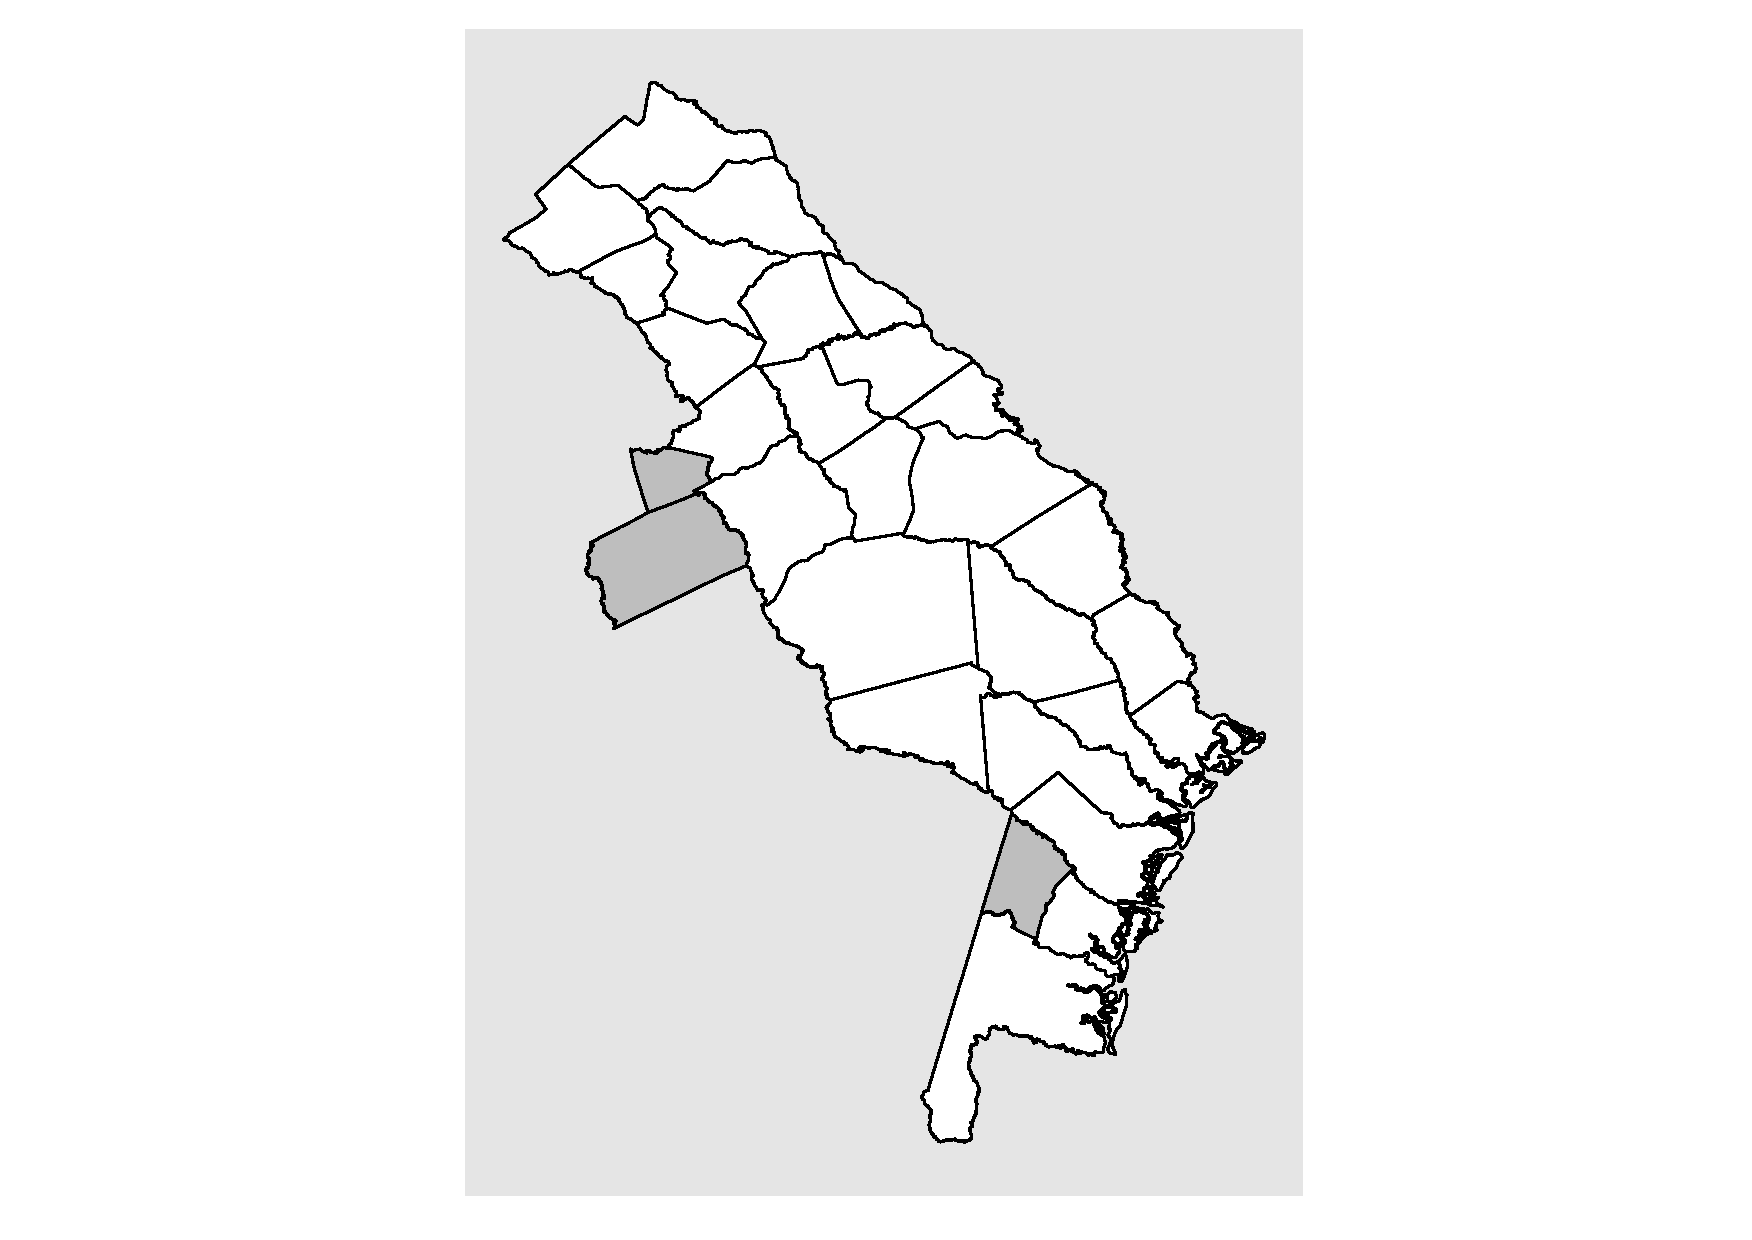
\includegraphics[width=4in]{county-map.pdf} 
   \caption{Map of Georgia with 1807 county boundaries \citep{long1995}. The northernmost shaded counties are Baldwin and Wilkinson, respectively, and Wayne is the southernmost shaded county.}
   \label{map}
\end{figure}
\end{frame}

\section[Data]{}

\begin{frame}
\frametitle{Data}
\begin{itemize}
\item List of 1805 lottery participants compiled by \citet{graham2005}
\item Fortunate drawer records for 1805 and 1807 lotteries \citep{graham2004,graham2011}
\item Roster of officeholders published by Georgia Archives (Trustee period -- 1847)
\item Roll call votes extracted from Journals of the House and Senate of the State of Georgia
\begin{itemize}
\item  15 votes: emancipate certain slaves; facilitate introduction of slaves into state and prevent slaves being carried out of the state; and punish slaves and free blacks
\end{itemize}
\item Individual property tax records (1790 -- 1865)  \citep{archives1890,blair1926}
\end{itemize}
\end{frame}

\begin{frame}
\frametitle{Linking participants with officeholders}
\begin{enumerate}
\item Manually deduplicate 1807 records matched with officeholders based on exact match of surname and Soundex codes of first name
\item Randomly split matched records into training (60\%) and test (40\%) sets
\item  Fit an algorithmic model using random forests \citep{breiman2001} on training set with features common to both datasets (test set error rate of 35\%)
\item Use model to deduplicate 1805 lottery records matched with officeholders
\end{enumerate}
\end{frame}

\section[Estimation]{}

\begin{frame}
\frametitle{Estimating treatment effects}
\begin{itemize}
\item \citet{neyman1923} framework: each $i = \left\{1, ..., N \right\}$ participants have two potential outcomes, $Y_{1i}$ and $Y_{0i}$
\item  $Z_i \in \{0,1\}$ denotes treatment assignment for $i$
\item Calculate weighted difference--in--means estimator for sample average treatment effect:

\begin{equation} \label{tstat}
\boldsymbol \delta^{*} = \frac{\sum_{i=1}^{N} (Y_{i} | Z_i = 1)}{n \mathrm{P} (Z_i = 1)}  -  \frac{\sum_{i=1}^{N} (Y_{i} | Z_i = 0)}{m(1-\mathrm{P} (Z_i = 1))},
\end{equation} where $n = \sum_{i=1}^{N} Z_i$, $m = N- n$, and 
\begin{align} \label{Z} 
\mathrm{P} (Z_i = 1) = \begin{cases}
\frac{\# \mathrm{Prizes}}{\# \mathrm{Tickets}} 	& \mbox{if} \, i \, \mathrm{has \, one \, draw}  \\
2 \left(\frac{\# \mathrm{Prizes}}{\# \mathrm{Tickets}}\right) 	& \mbox{if}\, i \, \mathrm{has \, two \, draws}.
\end{cases} 
\end{align} 
\end{itemize}
\end{frame}

\begin{frame}
\frametitle{Estimating treatment effects (cont.)}
\begin{itemize}
\begin{assumption}{1}{}\label{a1}
No interference between units: $Y_{i\boldsymbol Z}$ varies with $Z_i$, but does not vary with other elements of \textbf{Z}.
\end{assumption} 

\begin{assumption}{2}{}\label{a2}
Random treatment assignment: $\mathrm{P}(Z_i | Y_{i\boldsymbol Z}) = \mathrm{P}(Z_i)$ for all $i$. 
\end{assumption} 

\item Estimate exact two--sided $p$ value:

\begin{equation} \label{p} 
\hat{p} = \frac{\sum_{\mathcal{L}=1}^{\mathcal{L}} \boldsymbol Z \left(|\delta_\mathcal{L}| \geq |\delta^{*}|\right)}{\mathcal{L}},
\end{equation} where $\delta_\mathcal{L}$ is value of test statistic for $\mathcal{L}^{th}$ random sample from randomization distribution
\item CIs obtained by inverting randomization test
\end{itemize}
\end{frame}

\begin{frame}
\frametitle{Estimating treatment effects (cont.)}
\begin{itemize}
\item Noncompliance is an issue: 9\% in 1805 sample and 22\% in combined sample
\item Implement \citet{angrist1996} IV procedure: $Z_i$ instruments for $D_i (\boldsymbol Z) \in\{0,1\}$ indicating if treatment actually received
\begin{assumption}{3}{}\label{a5}
No defiers: $D_i (1) \geq D_i (0) =0 \hspace{5mm} \forall \,i.$
\end{assumption} 
\item Average causal effect on compliers:
\begin{align}
\frac{\E [Y_i  | Z_i = 1] - \E[Y_i | Z_i = 0]}{\E[D_i (1)]} \\ \nonumber
= \E[Y_{1i} - Y_{0i} | D_i (1)=1] \label{LATE}
\end{align} 
\end{itemize}
\end{frame}

\section[Balance for 1805 sample]{}

%Balance plot
\begin{frame}
\begin{figure}[htbp]
%\caption{Balance in treatment assignment for 1805 sample.}
\begin{center}
   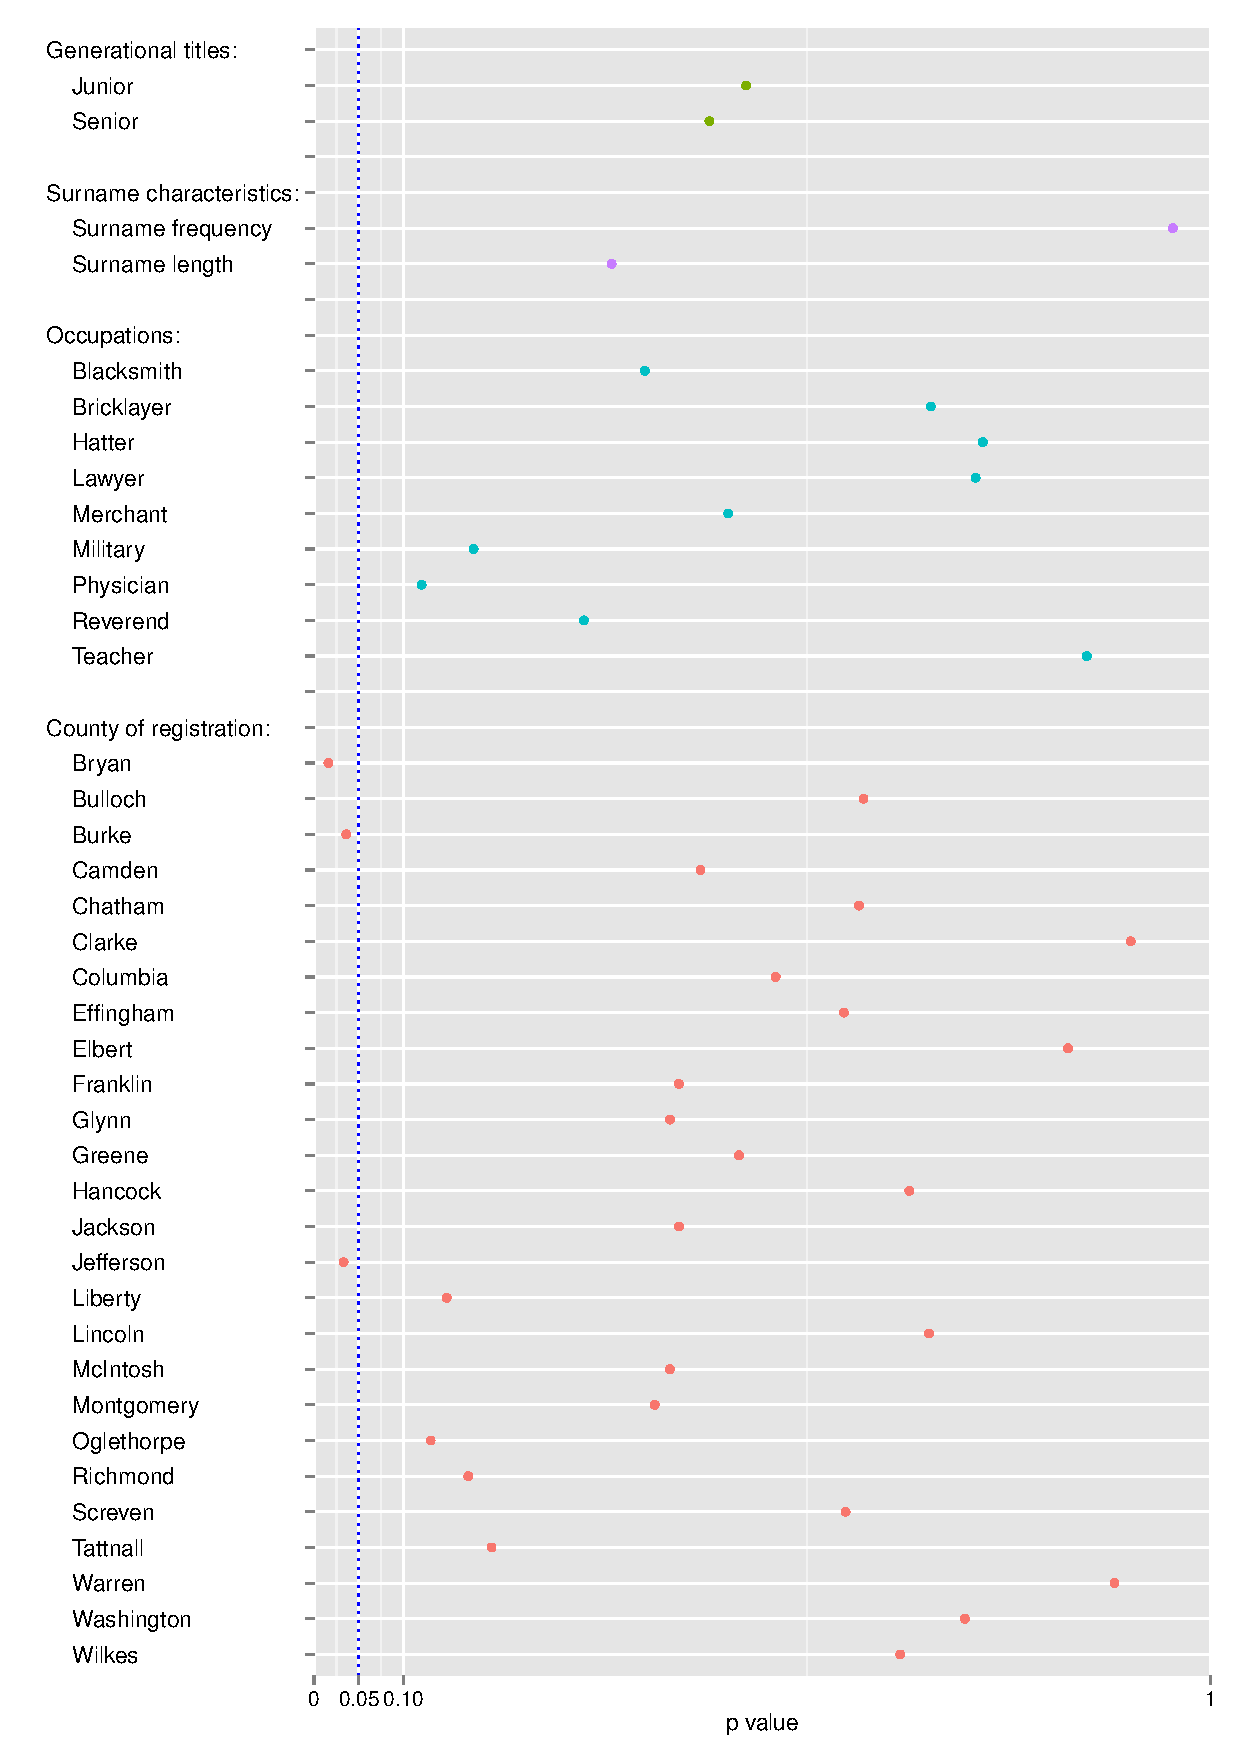
\includegraphics[width=0.50\linewidth]{balance-plot.pdf} 
  \end{center}
 %  \footnotesize{Note: $p$ values are calculated using a two--sided randomization test ($\mathcal{L}=1,000$ iterations) for weighted difference of means between treatment and control groups. Refer to footnotes in Table \ref{balance-nom} and Figure \ref{qq} for variable descriptions.}
\label{balance-plot}
\end{figure}
\end{frame}

\section[Results]{}

%Treatment effect on officeholding
\begin{frame}
\frametitle{Results}
\begin{table}[htb]
\caption{Officeholding by treatment assignment.}   \label{lotteries} 
  \begin{tabularx}{\linewidth}{l*{8}{Y}}
    \toprule
    \multicolumn{8}{l}{\textbf{Panel A: 1805 sample}} \\
    \midrule
\textbf{Response}&  & $\textbf{Control}$ & $\mathbf{\%_{\mathrm{m}}}$ & $\textbf{Treated}$ & $\mathbf{\%_{\mathrm{n}}}$ & $\textbf{All}$ & $\mathbf{\%_{\mathrm{N}}}$ \\ 
  \hline
Officeholder & 0 & 16747 & 93.1 & 3058 & 93.2 & 19805 & 93.2 \\ 
   & 1 & 1234 & 6.9 & 222 & 6.8 & 1456 & 6.8 \\ 
   \hline
 & all & 17981 & 100.0 & 3280 & 100.0 & 21261 & 100.0 \\ 
  \end{tabularx}
  \begin{tabularx}{\linewidth}{l*{8}{Y}}
    \toprule
    \multicolumn{8}{l}{\textbf{Panel B: Combined sample}} \\
    \midrule
Officeholder & 0 & 16747 & 93.1 & 10813 & 93.9 & 27560 & 93.4 \\ 
   & 1 & 1234 & 6.9 & 705 & 6.1 & 1939 & 6.6 \\ 
   \hline
 & all & 17981 & 100.0 & 11518 & 100.0 & 29499 & 100.0 \\ 
    \bottomrule
  \end{tabularx}
 \footnotesize{Notes: Distribution of officeholders by treatment assignment for sample of 1805 lottery participants (Panel A) and combined sample of 1805 participants and 1807 fortunate drawers (Panel B). Both samples exclude women orphans, and pretreatment officeholders.}
\end{table}
\end{frame}

%Treatment effect on support for slavery
\begin{frame}
\frametitle{Results (cont.)}
\begin{table}[htb]
\caption{Support for slavery by treatment assignment.}   \label{outcomes-assembly}
  \begin{tabularx}{\linewidth}{l*{8}{Y}}
    \toprule
    \multicolumn{8}{l}{\textbf{Panel A: 1805 sample}} \\
    \midrule
 \textbf{Variable} & \textbf{Treatment} & $\mathbf{N}$ & \textbf{Min.} & $\mathbf{Mean}$ & \textbf{Max.} & $\mathbf{S.d.}$ & \textbf{\#NA}\\ 
  \hline
Support for slavery & 0 & 255 & 0 & 0.737 & 1 & 0.366 &  963 \\ 
   & 1 & 219 & 0 & 0.722 & 1 & 0.382 &  632 \\ 
   \hline
 & all & 474 & 0 & 0.730 & 1 & 0.373 & 1595 \\ 
   \hline
  \end{tabularx}
  \begin{tabularx}{\linewidth}{l*{8}{Y}}
    \toprule
    \multicolumn{8}{l}{\textbf{Panel B: Combined sample}} \\
    \midrule
Support for slavery & 0 & 401 & 0 & 0.735 & 1 & 0.371 & 1353 \\ 
   & 1 & 216 & 0 & 0.757 & 1 & 0.369 &  763 \\ 
   \hline
 & all & 617 & 0 & 0.743 & 1 & 0.370 & 2116 \\ 
    \bottomrule
  \end{tabularx} \\
\footnotesize{Distribution of the outcome variable, by treatment assignment, for 1805 participants (Panel A) or combined sample of 1805 participants and 1807 fortunate drawers (Panel B) who held office in the General Assembly before 1848 . `Support for slavery' is the mean of votes in favor of slavery.} 
\end{table}
\end{frame}

%Summary of results
\begin{frame}
\frametitle{Results (cont.)}
\begin{figure}[htbp]
\begin{center}
 %     \caption{Treatment effect estimates for each hypothesis test and sample used (horizontal lines represent 95\% confidence intervals)}
   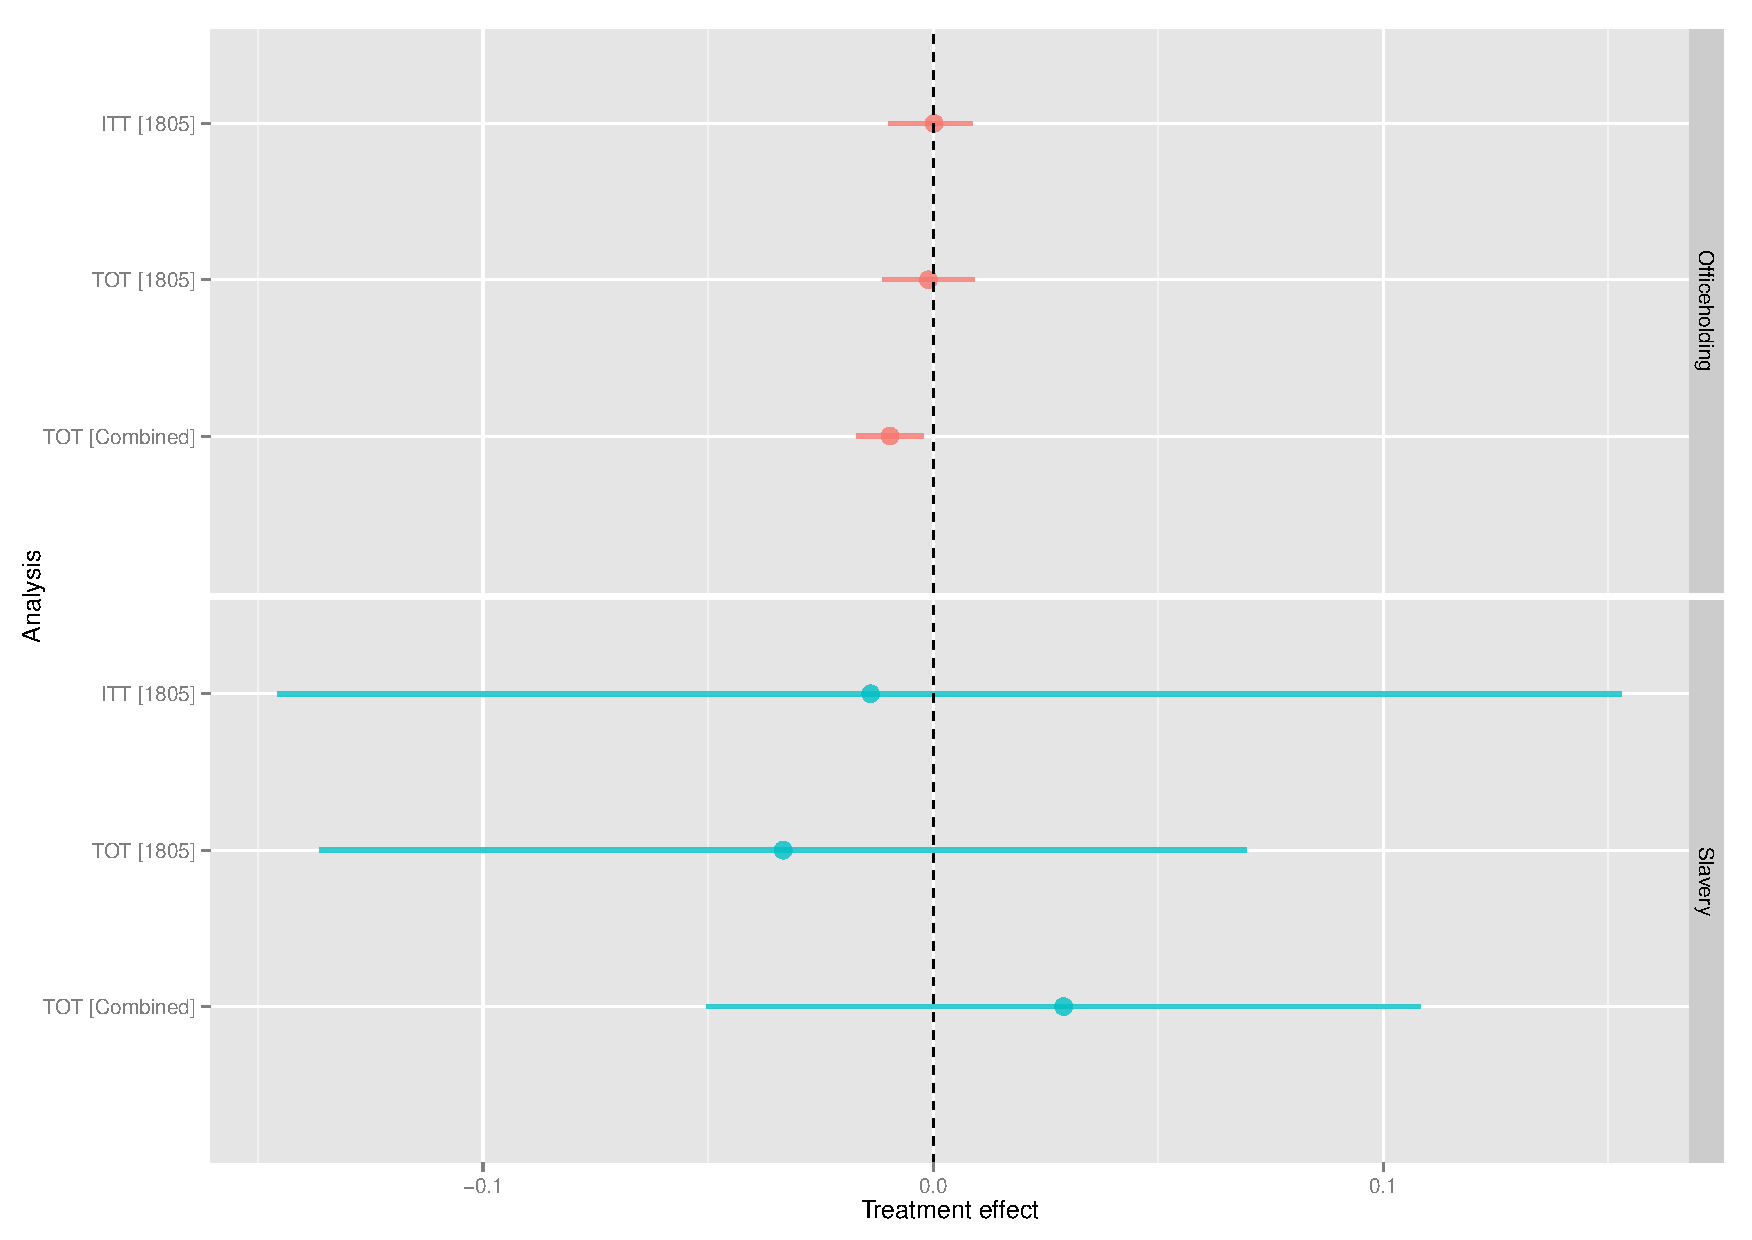
\includegraphics[scale=0.37]{forest-plot.pdf} 
   \label{forest-plot} \\
   \end{center}
\end{figure}
\end{frame}

\section[Heterogeneous treatment effects]{}

\begin{frame}
\begin{figure}[htbp]
\begin{center}
      \caption{Heterogenous treatment effects for 1805 lottery participants.}
   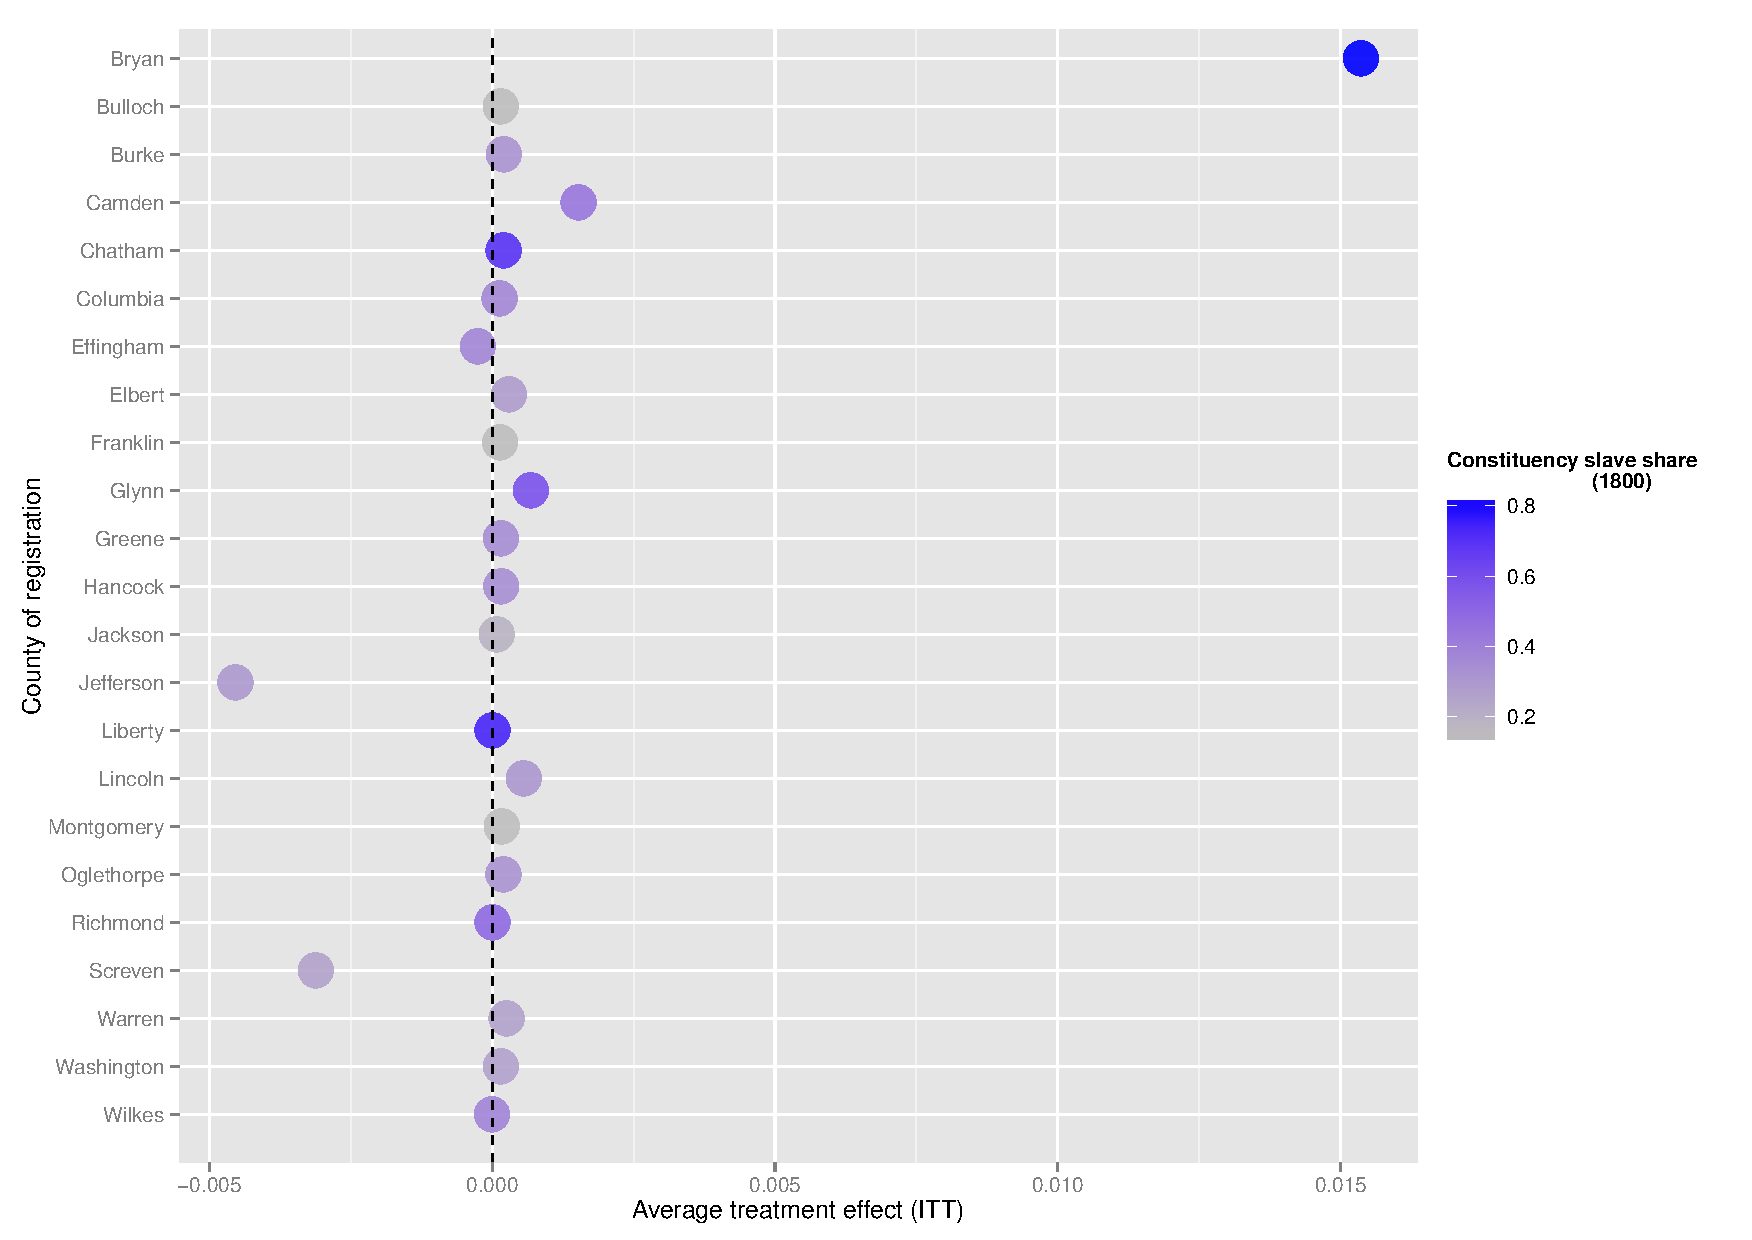
\includegraphics[scale=0.35]{het-plot-oh.pdf} 
   \label{het-plot-oh}
   \end{center}
\end{figure}
\end{frame}

%Wealth densitiies
\begin{frame}
\begin{figure}[htbp]
\begin{center}
      \caption{Pre-- and posttreatment wealth densities for legislator--participants who voted on roll calls.}
   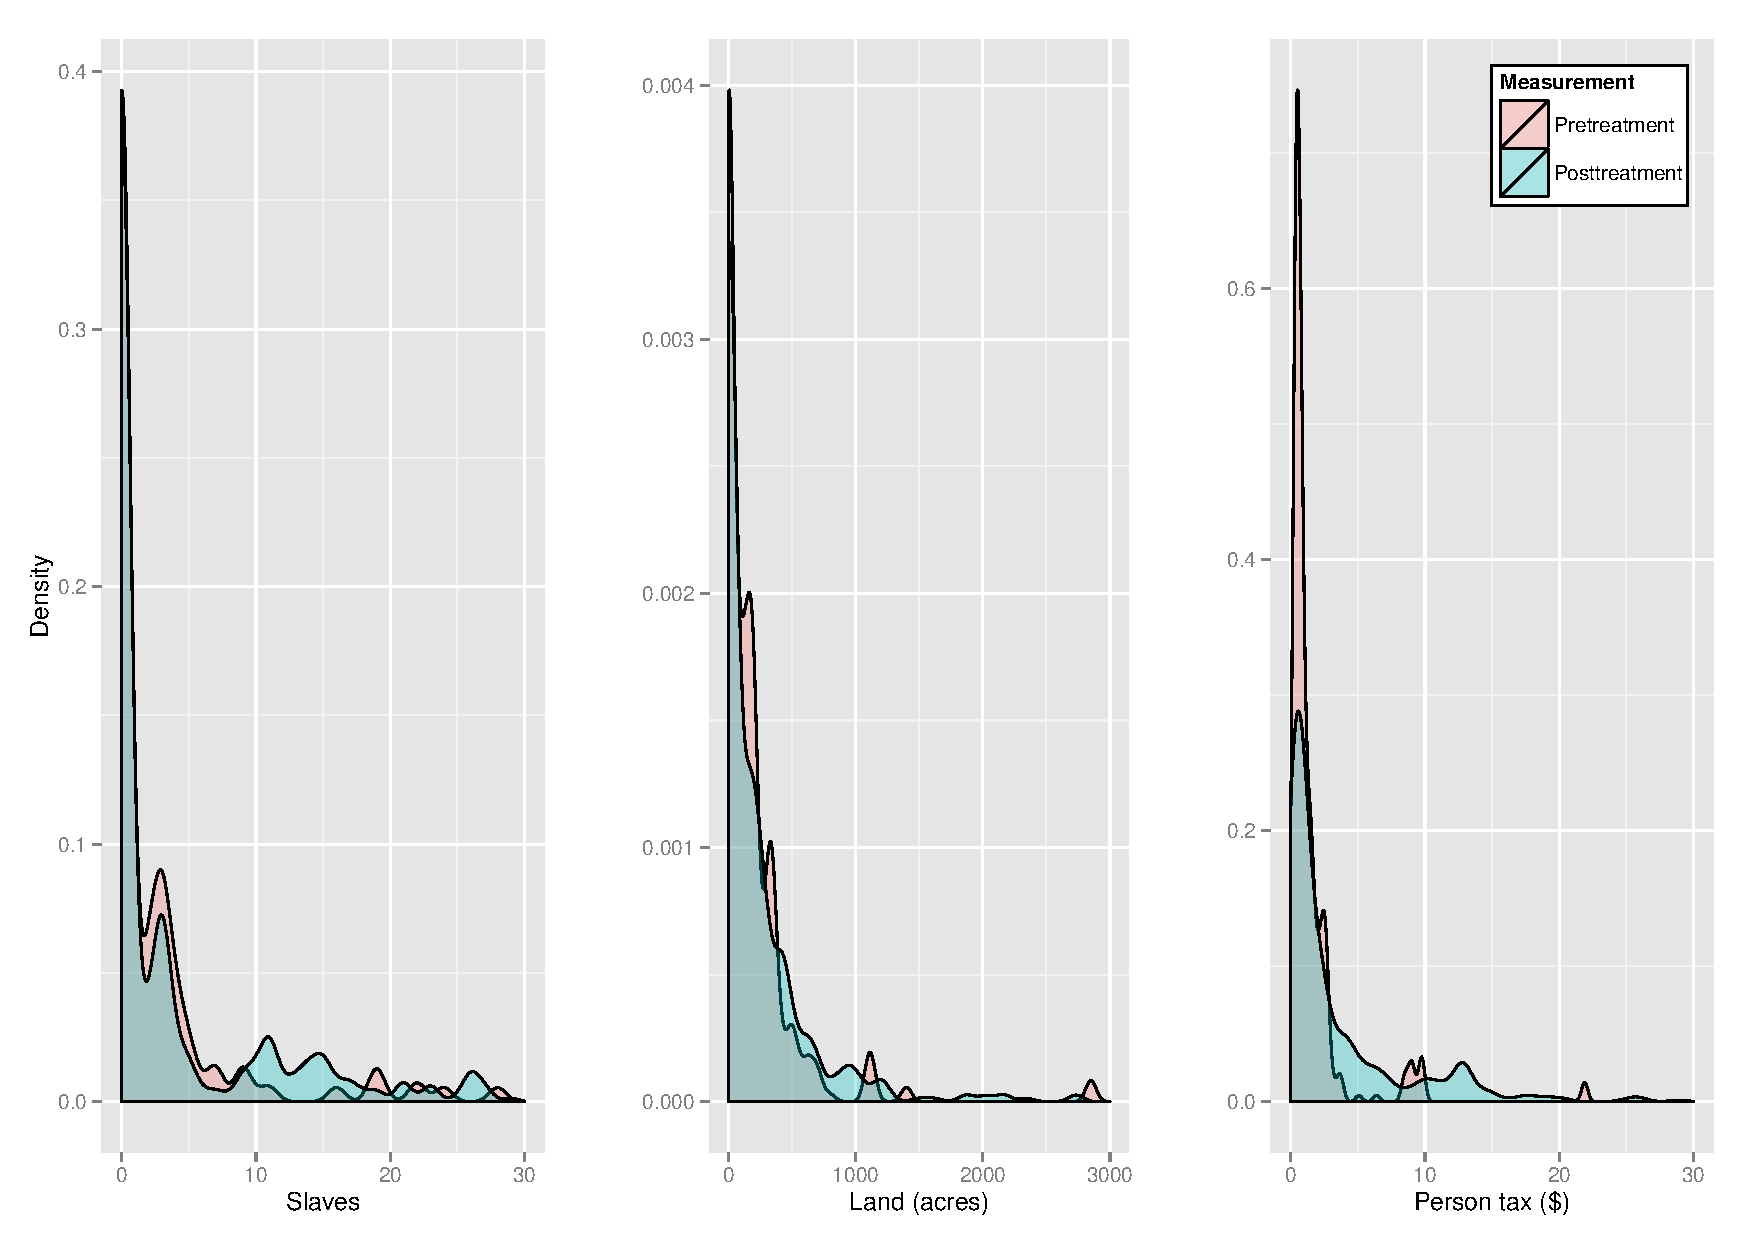
\includegraphics[scale=0.33]{wealth-plot.pdf} 
   \label{wealth-plot}
   \end{center}
\end{figure}
\end{frame}

\begin{frame}
\begin{figure}[htbp]
\begin{center}
      \caption{Heterogenous treatment effects for legislators who voted on roll calls.}
   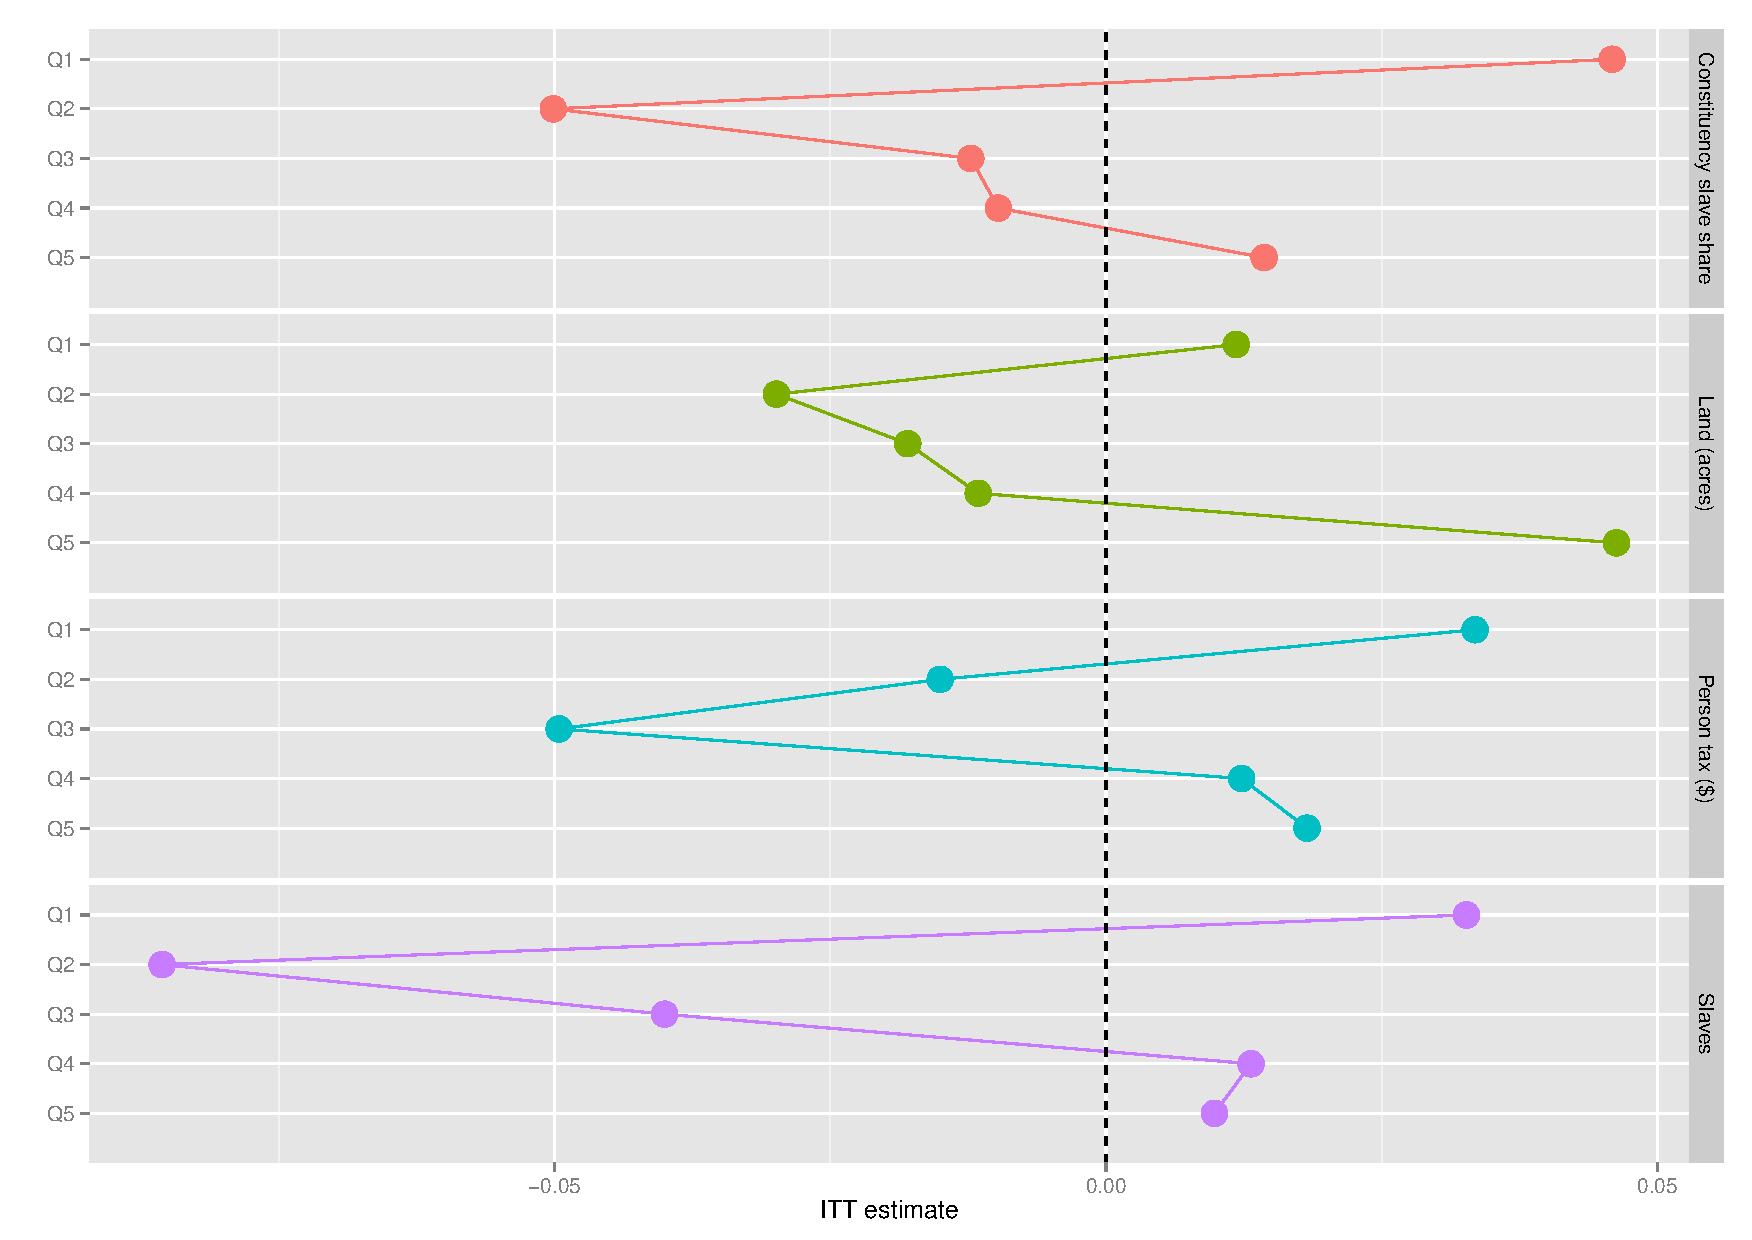
\includegraphics[scale=0.35]{het-plot-assembly.pdf} 
   \label{het-plot-assembly}
   \end{center}
\end{figure}
\end{frame}

\section[Discussion]{}

\begin{frame}
\frametitle{Discussion}
\begin{itemize}
\item If property wealth influences political power, we should be able to find evidence in antebellum South
\item Officeholding: tight CIs on zero effect implies evidence ``in favor of'' null
\item Elite ideology: too much uncertainty to detect significant treatment effect
\begin{itemize}
\item Substantial heterogeneity in treatment effect according to pretreatment wealth
\end{itemize}
\end{itemize}
\end{frame}

\section[References]{}

\begin{frame}
\begin{singlespace}
\begin{tiny}
\bibliographystyle{plainnat}
\bibliography{references}
\end{tiny}
\end{singlespace}
\itemize
\end{frame}

		
\end{document}

